\chapter{Lab 8: Memory} \label{day8}

\section{Memory module}

This module can store and output stored information. The data to be stored is received using the ``UART''-receiver module from the previous lab and then read out from the memory and displayed on the display of the \gls{fpga} board after pressing a button. 

The module can store 256 bytes. After 256 bytes the write address overflows and starts to overwrite information. The read address can be selected with switches and displayed after pressing a button.

\lstinputlisting[language=VHDL]{./L8/E1/src/project_8_1.vhd}

\lstinputlisting[language=VHDL]{./L8/E1/src/project_8_1_1.vhd}

\section{LIFO/stack}

The ``LIFO'' stack works as follows: The last stored information ist the first to be output. We use it here to display the received information from the computer keyboard on the display of the \gls{fpga} after pressing the button.

\lstinputlisting[language=VHDL]{./L8/E2/src/project_8_2.vhd}

\lstinputlisting[language=VHDL]{./L8/E2/src/project_8_2_1.vhd}

Additionally we test several borderline cases: 

\begin{itemize}
    \item reading from an empty stack
    \item writing to a full stack
    \item simultaneous reading and writing (starting with a full/empty stack)
\end{itemize}

\begin{figure}
    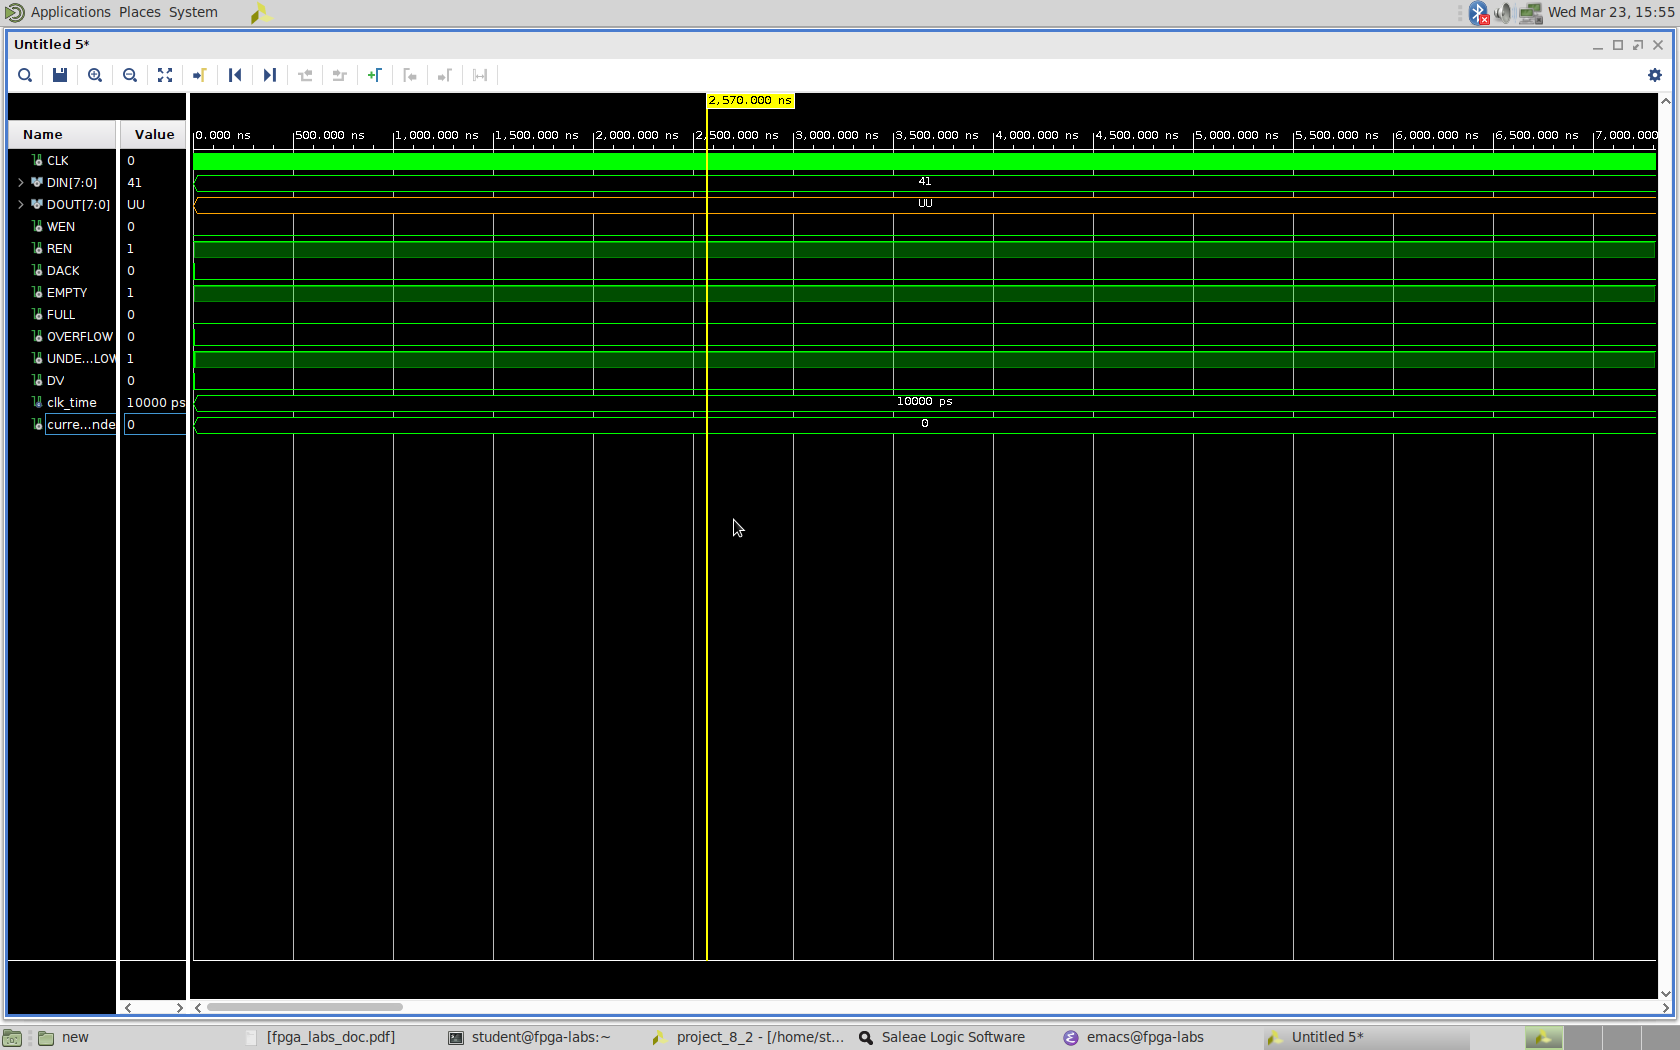
\includegraphics[width=.9\textwidth]{L8/E2/underflow.png}
    \caption{Reading from an empty stack. The stack underflows.}
    \label{pic: reading from an empty stack}
\end{figure}

\begin{figure}
    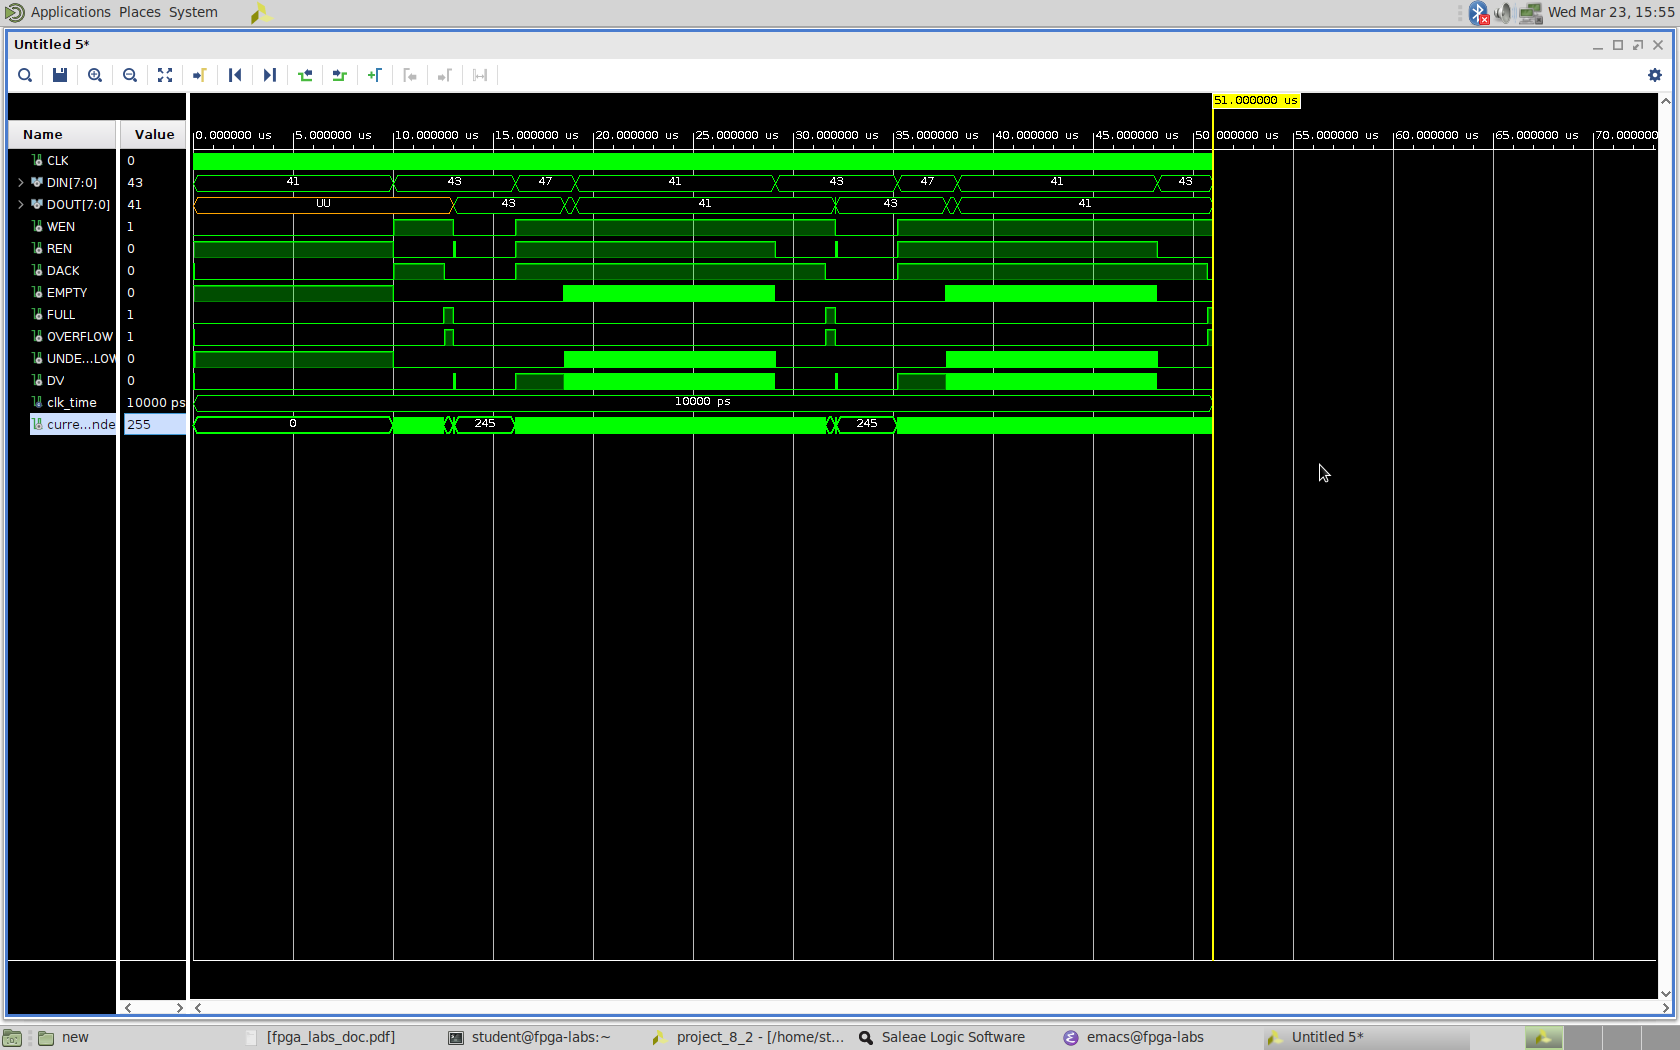
\includegraphics[width=.9\textwidth]{L8/E2/full.png}
    \caption{Writing to a full stack. The stack overflows and information is overwritten.}
    \label{pic: writing to a full stack}
\end{figure}

\begin{figure}
    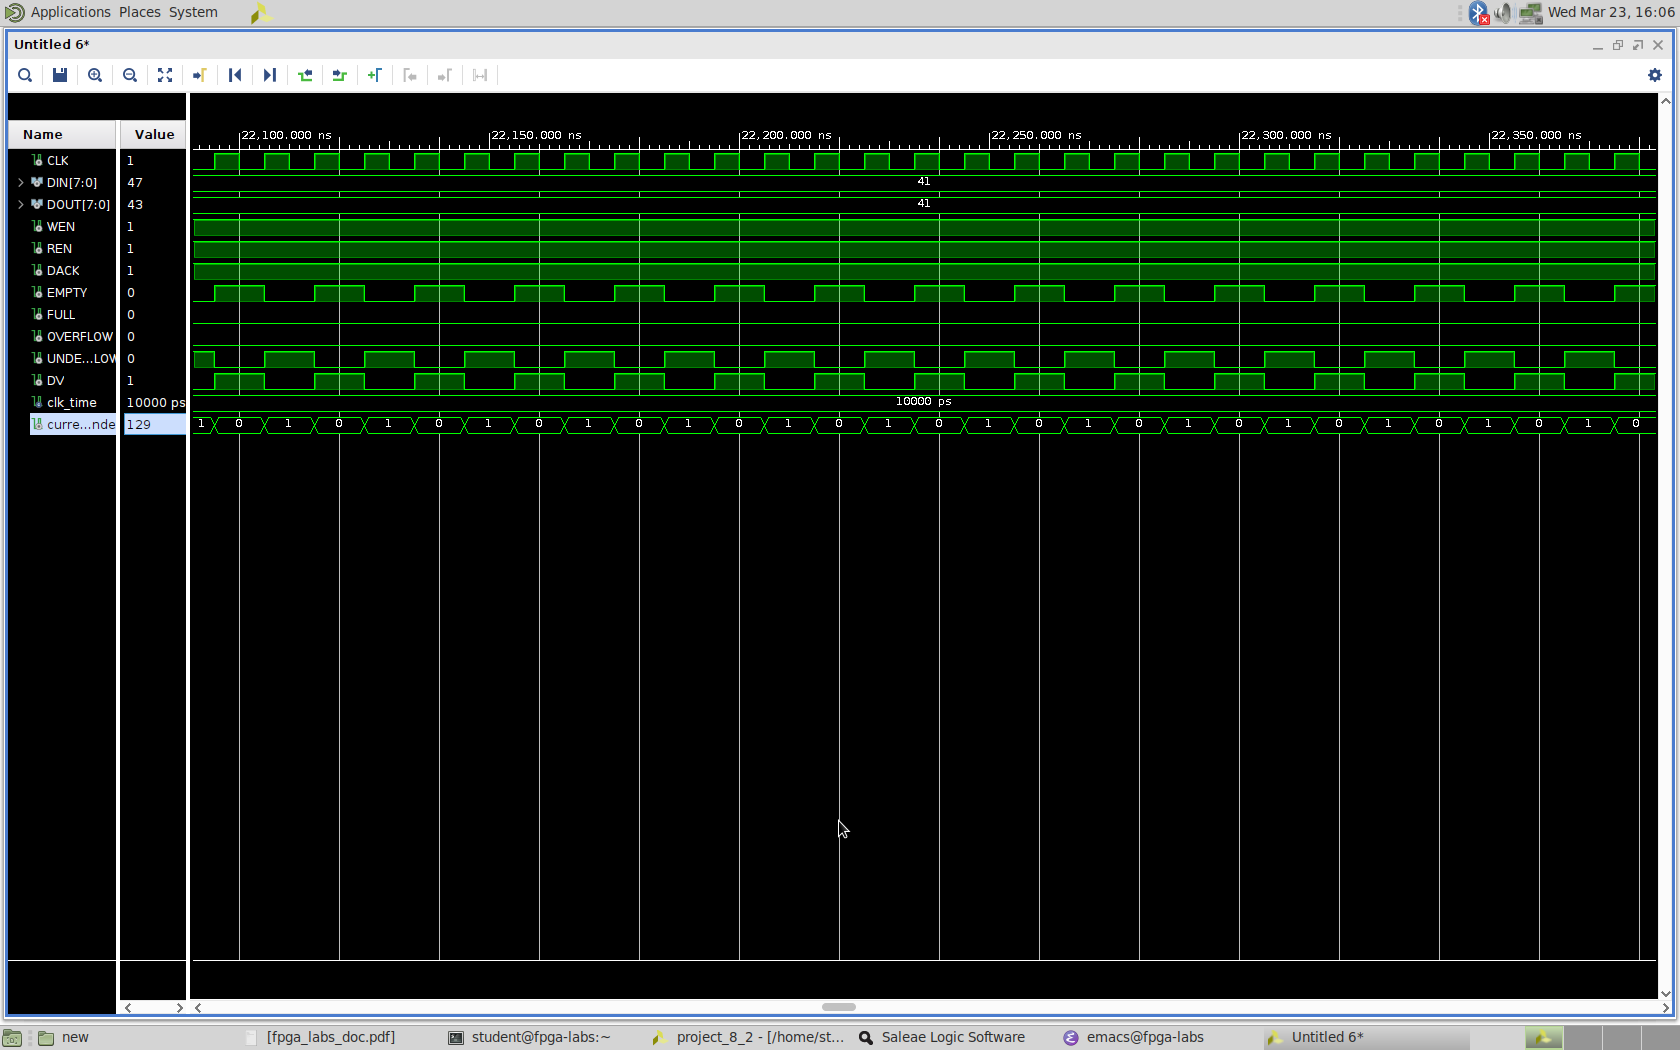
\includegraphics[width=.9\textwidth]{L8/E2/sim_read_write_underflow_empty.png}
    \caption{Writing and reading from an empty stack. The current address number oscillates between 0 and 1.}
    \label{pic: w and r from e stack}
\end{figure}

\begin{figure}
    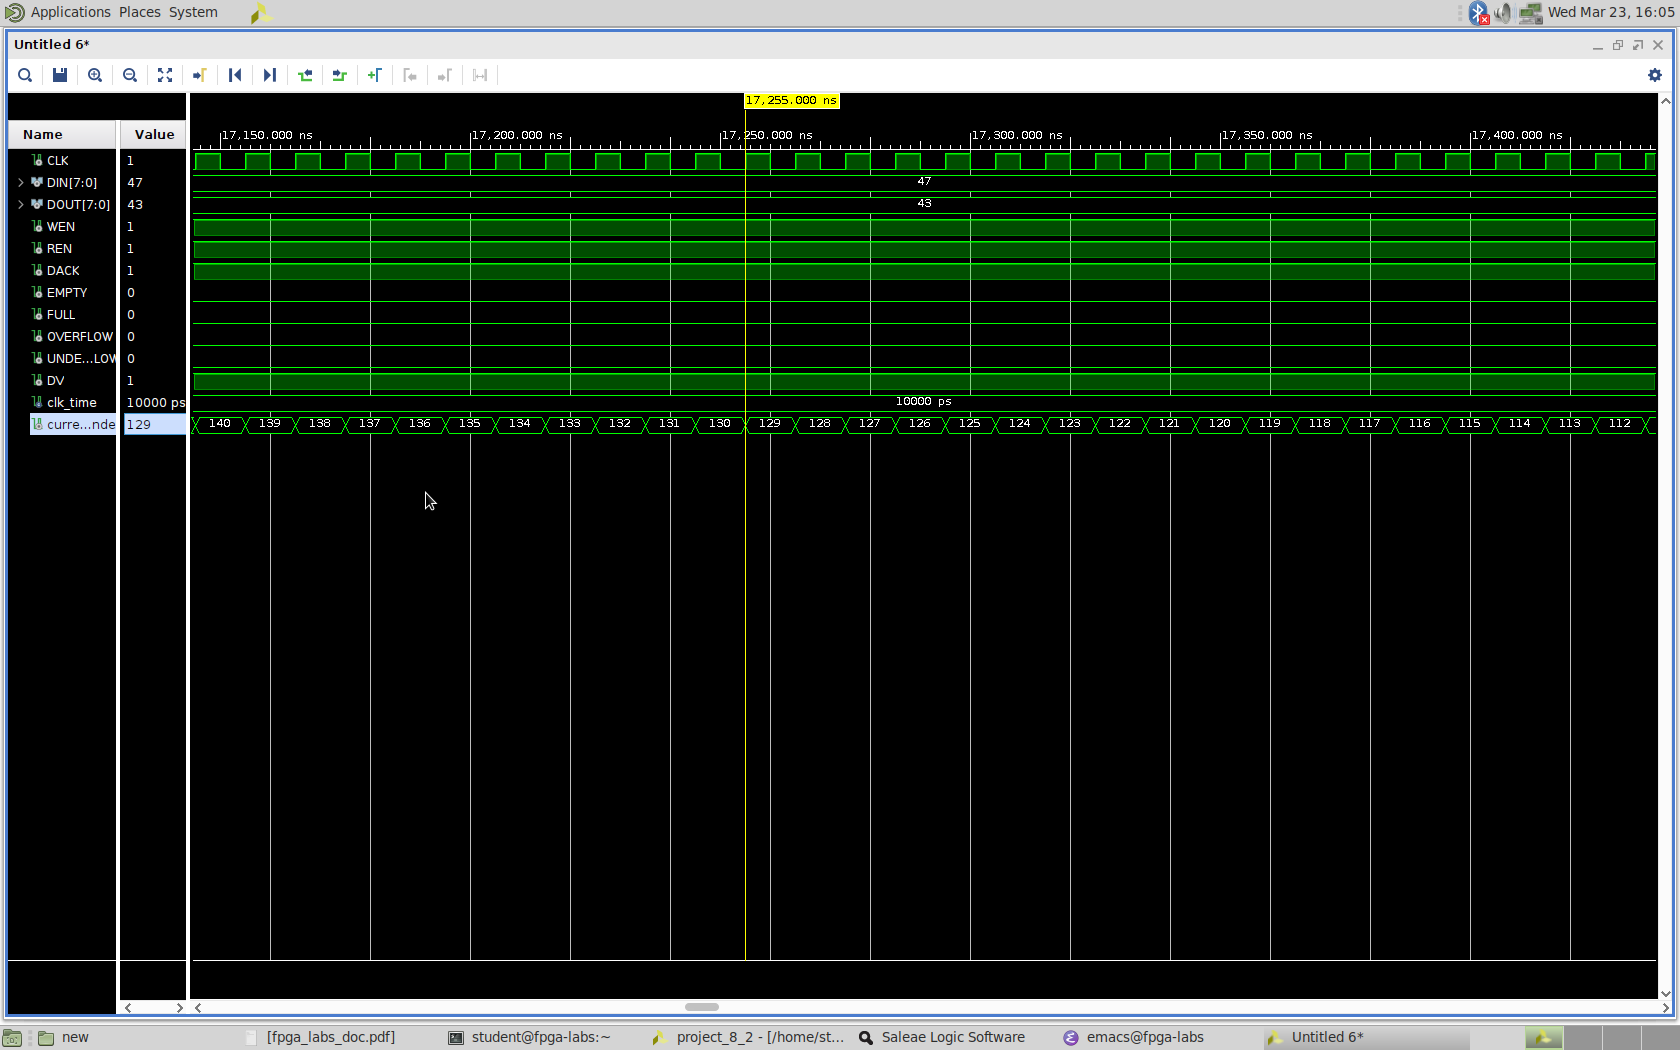
\includegraphics[width=.9\textwidth]{L8/E2/sim_read_write_full.png}
    \caption{Writing and reading from a full stack. The current address number goes down.}
    \label{pic: w and r from f stack}
\end{figure}

\newpage

\section{FIFO/queue}

The FIFO or queue module outputs the information in the exact order initially input to the memory. This is done with two pointers. One pointer for the input and one for the output.

\lstinputlisting[language=VHDL]{L8/E3/src/project_8_3.vhd}

\lstinputlisting[language=VHDL]{L8/E3/src/project_8_2_1.vhd}

\lstinputlisting[language=VHDL]{L8/E3/src/project_8_2_tb.vhd}

Again we simulated the borderline cases:

\begin{figure}
    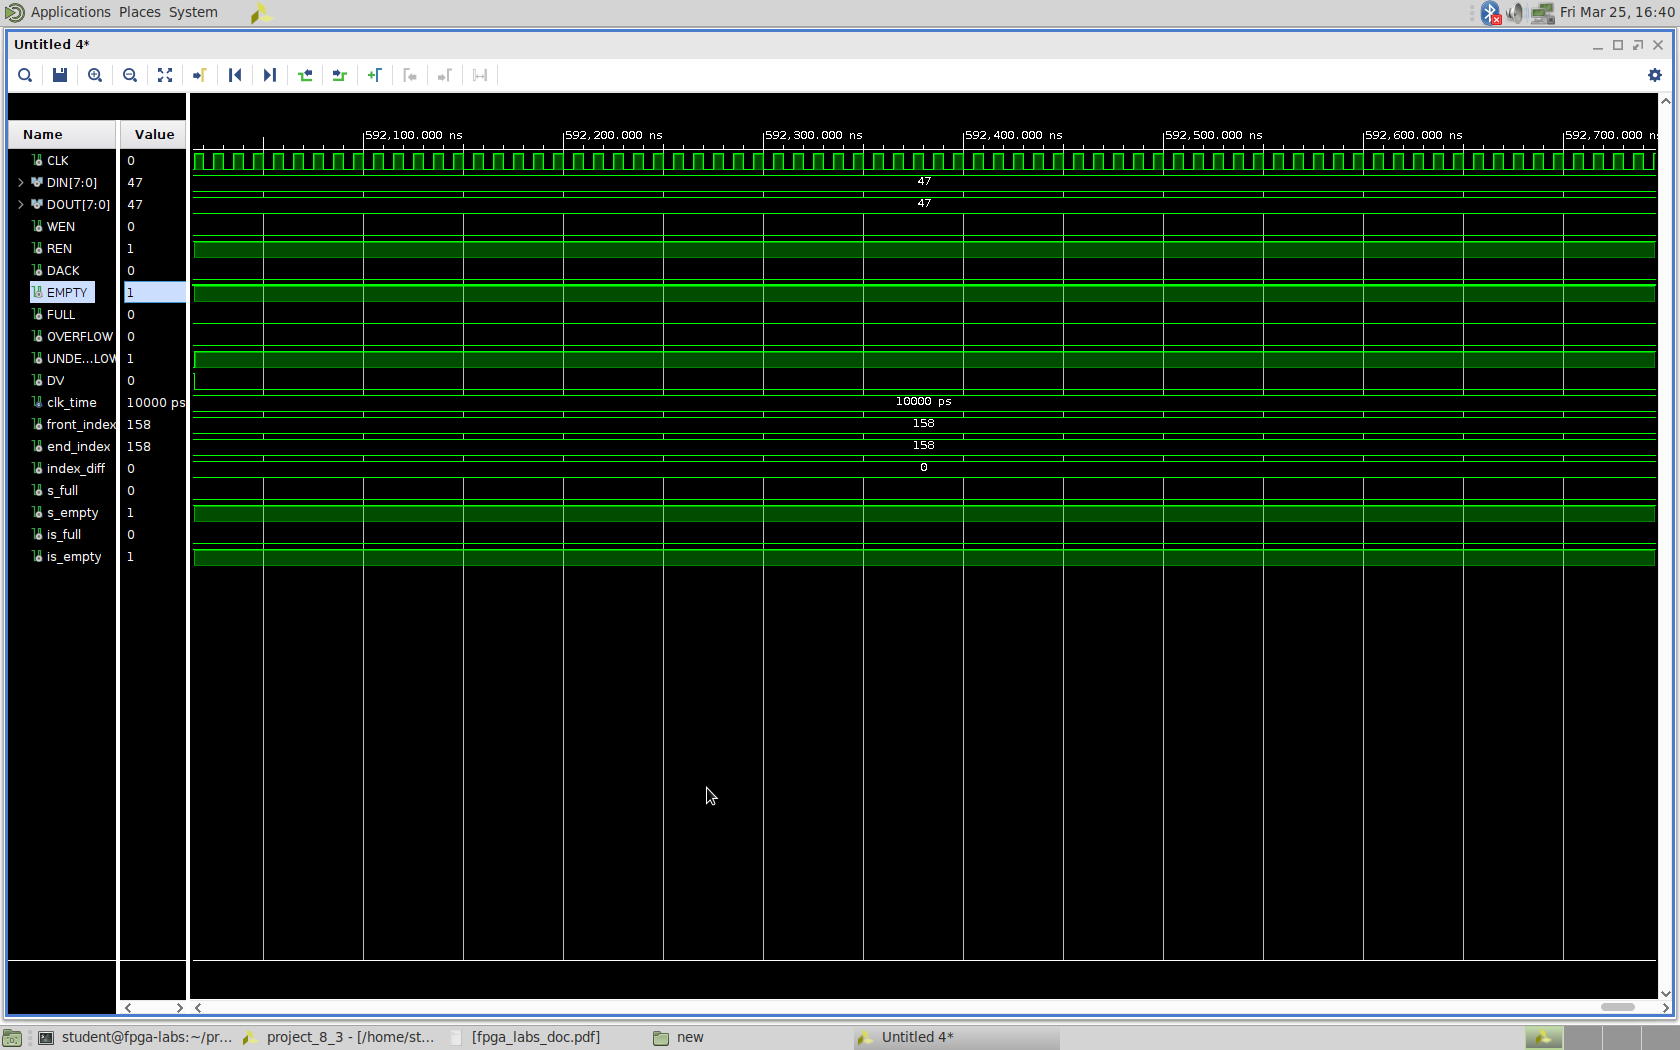
\includegraphics[width=.9\textwidth]{L8/E3/empty_read.png}
    \caption{Reading from an empty stack. The module returns that it is empty and underflows.}
    \label{pic: r from e stack fifo}
\end{figure}

\begin{figure}
    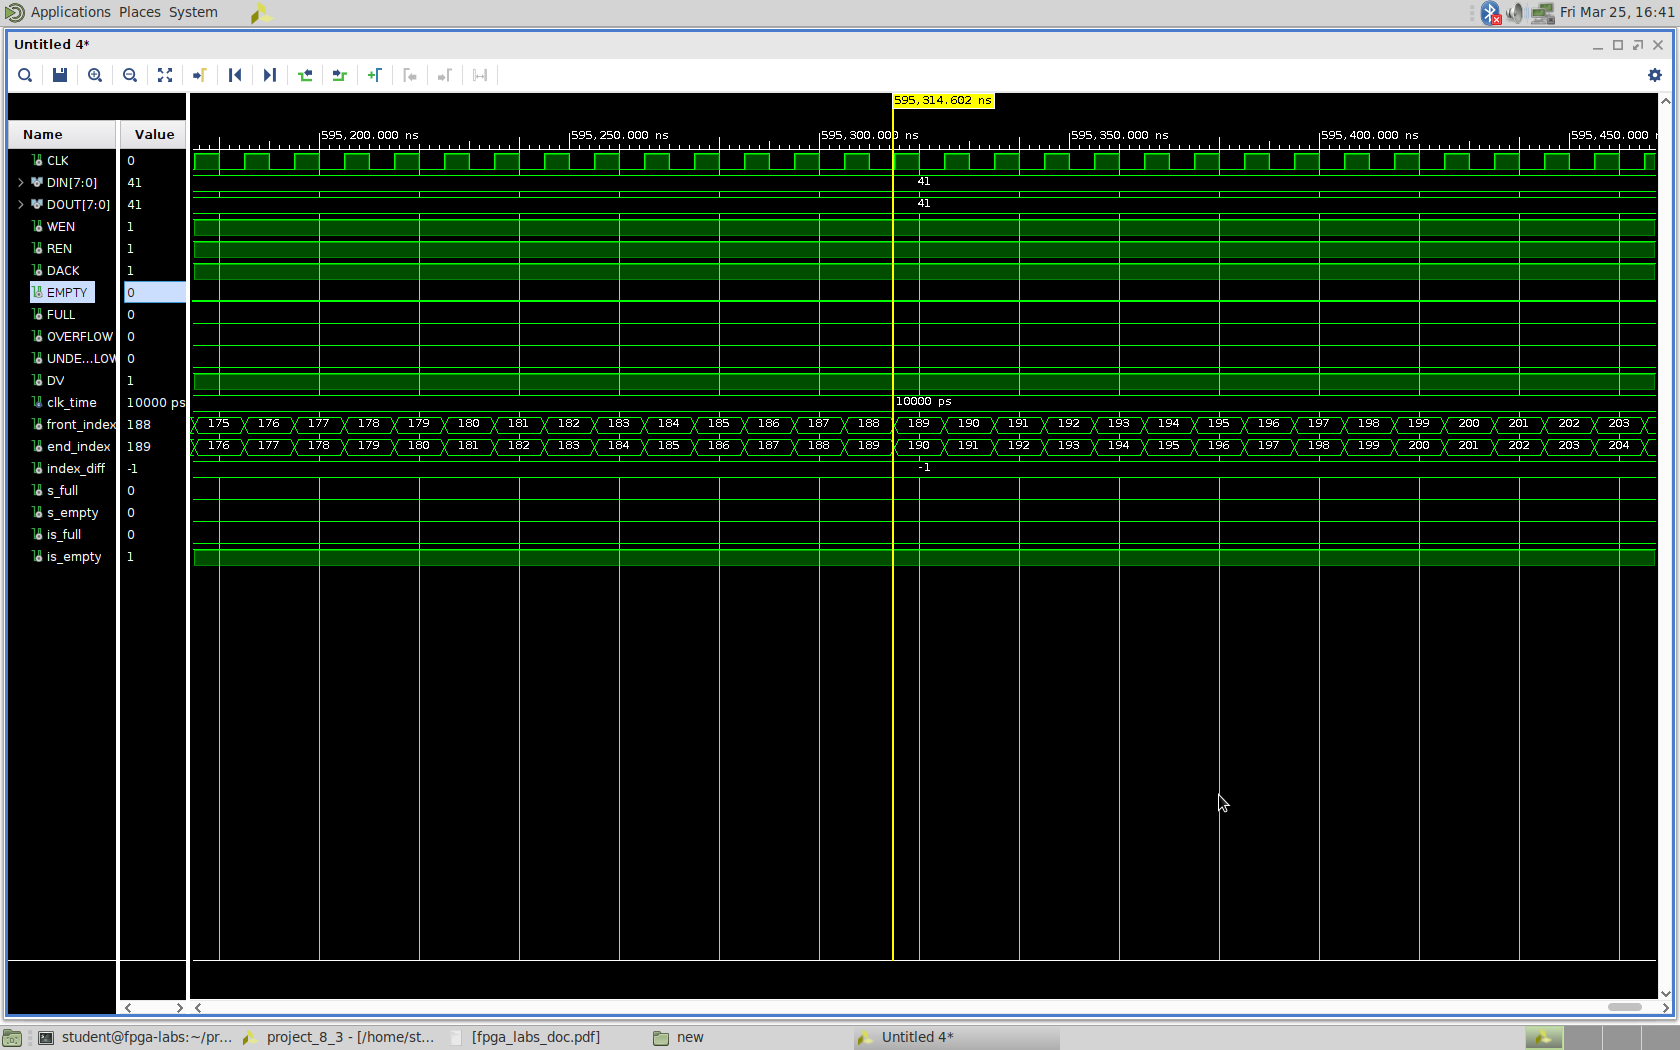
\includegraphics[width=.9\textwidth]{L8/E3/read_and_write_sametime.png}
    \caption{Simultaneous reading an writing. The module writes and reads correctly at the same time.}
    \label{pic: r and e from half stack fifo}
\end{figure}

\begin{figure}
    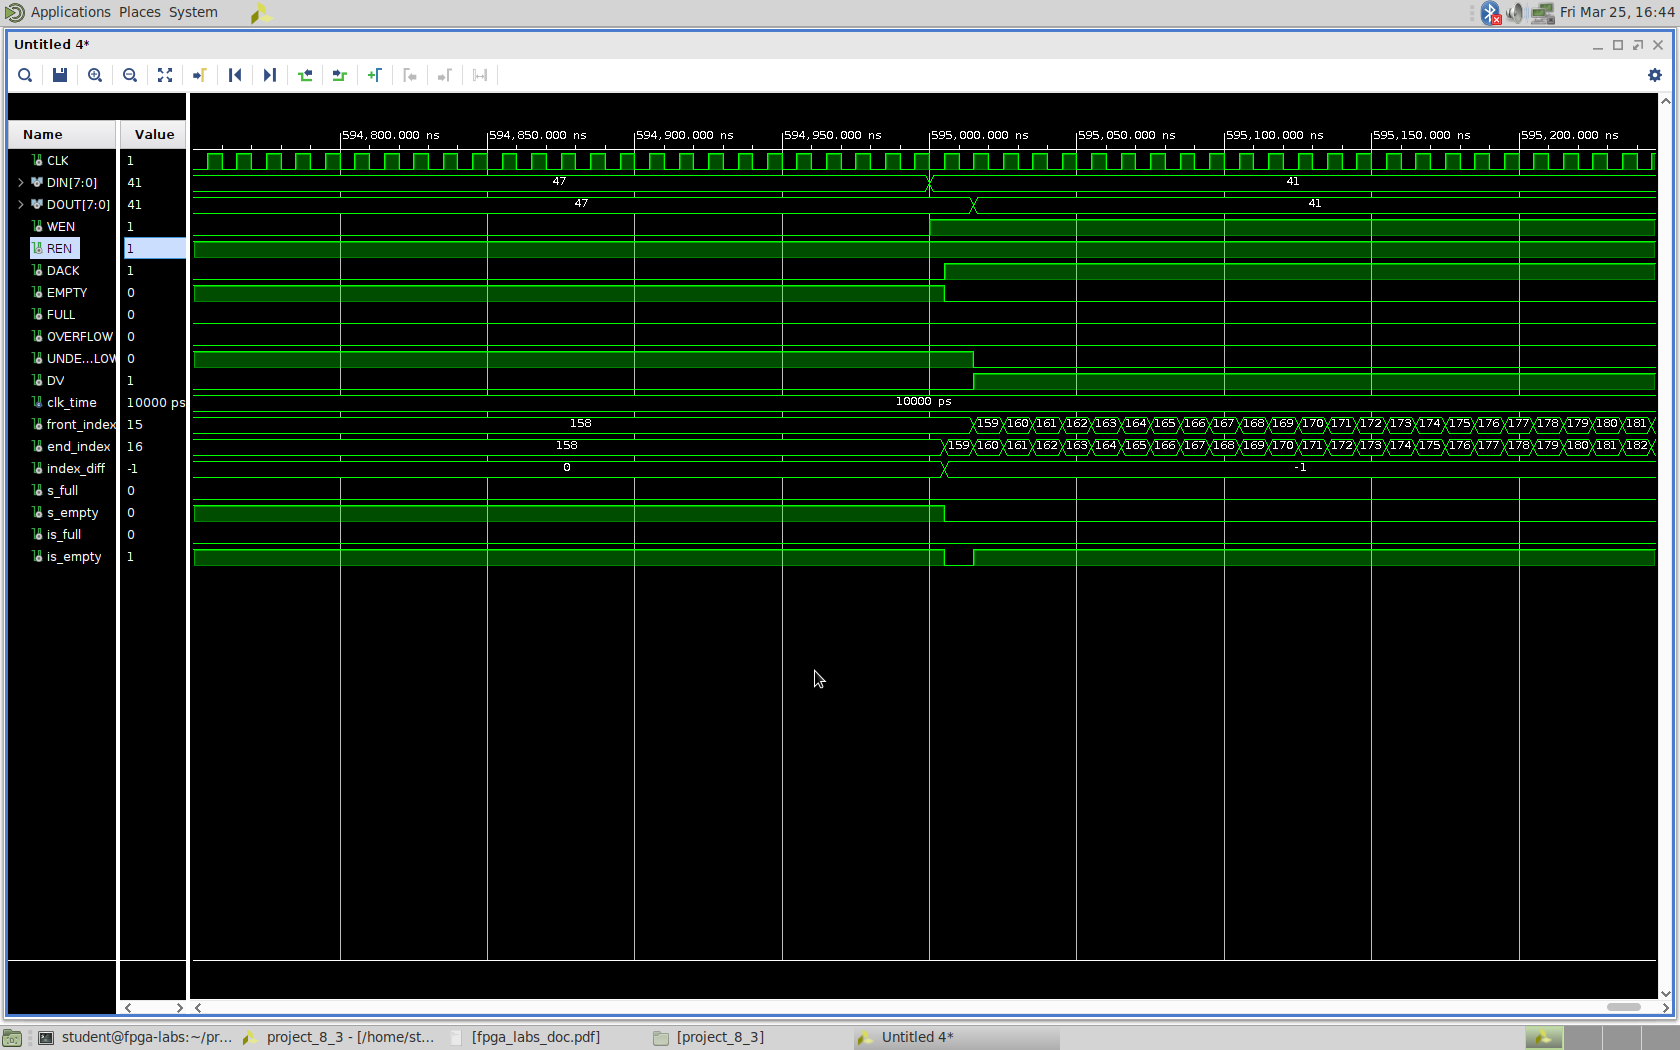
\includegraphics[width=.9\textwidth]{L8/E3/read_write_from_empty.png}
    \caption{Simultaneous reading an writing from empty stack. The end index (which is used as the write index) moves one up and the front index stays the same. It then shows the same behavior as before.}
    \label{pic: r and e from e stack fifo}
\end{figure}

\begin{figure}
    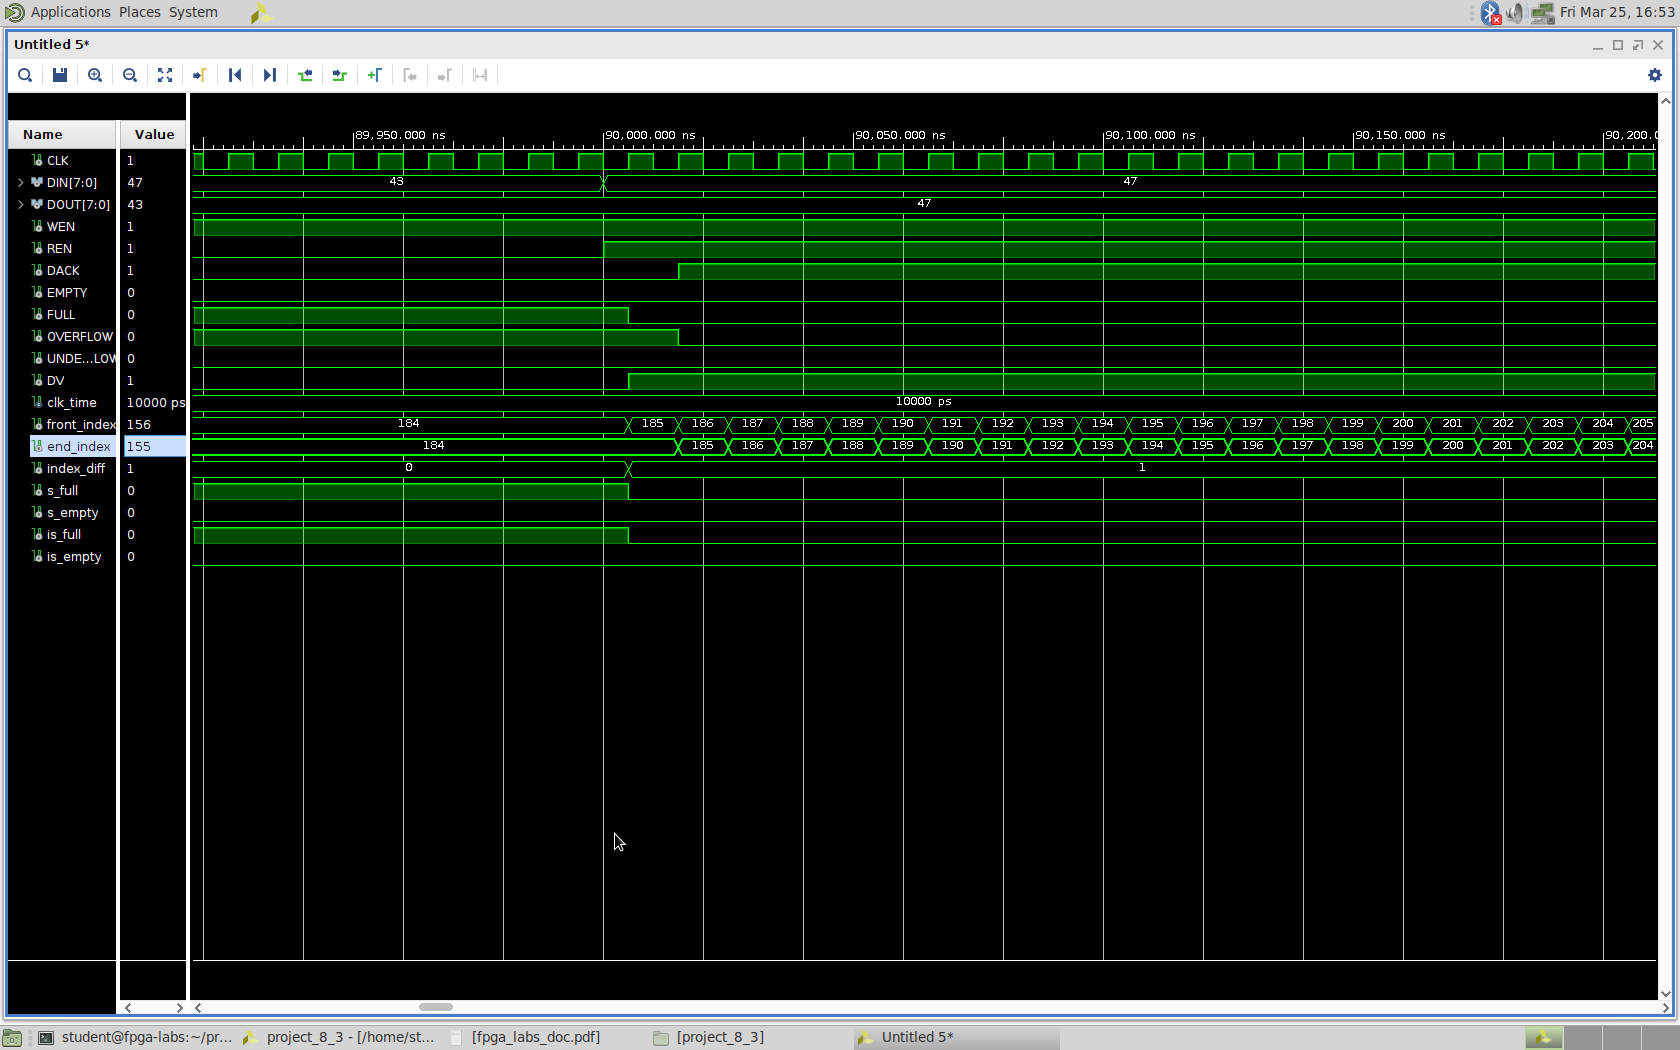
\includegraphics[width=.9\textwidth]{L8/E3/read_write_from_full.png}
    \caption{Simultaneous reading an writing from full stack. Here, the read index moves first and as free space is available again the write index moves upwards.}
    \label{pic: r and e from f stack fifo}
\end{figure}

\begin{figure}
    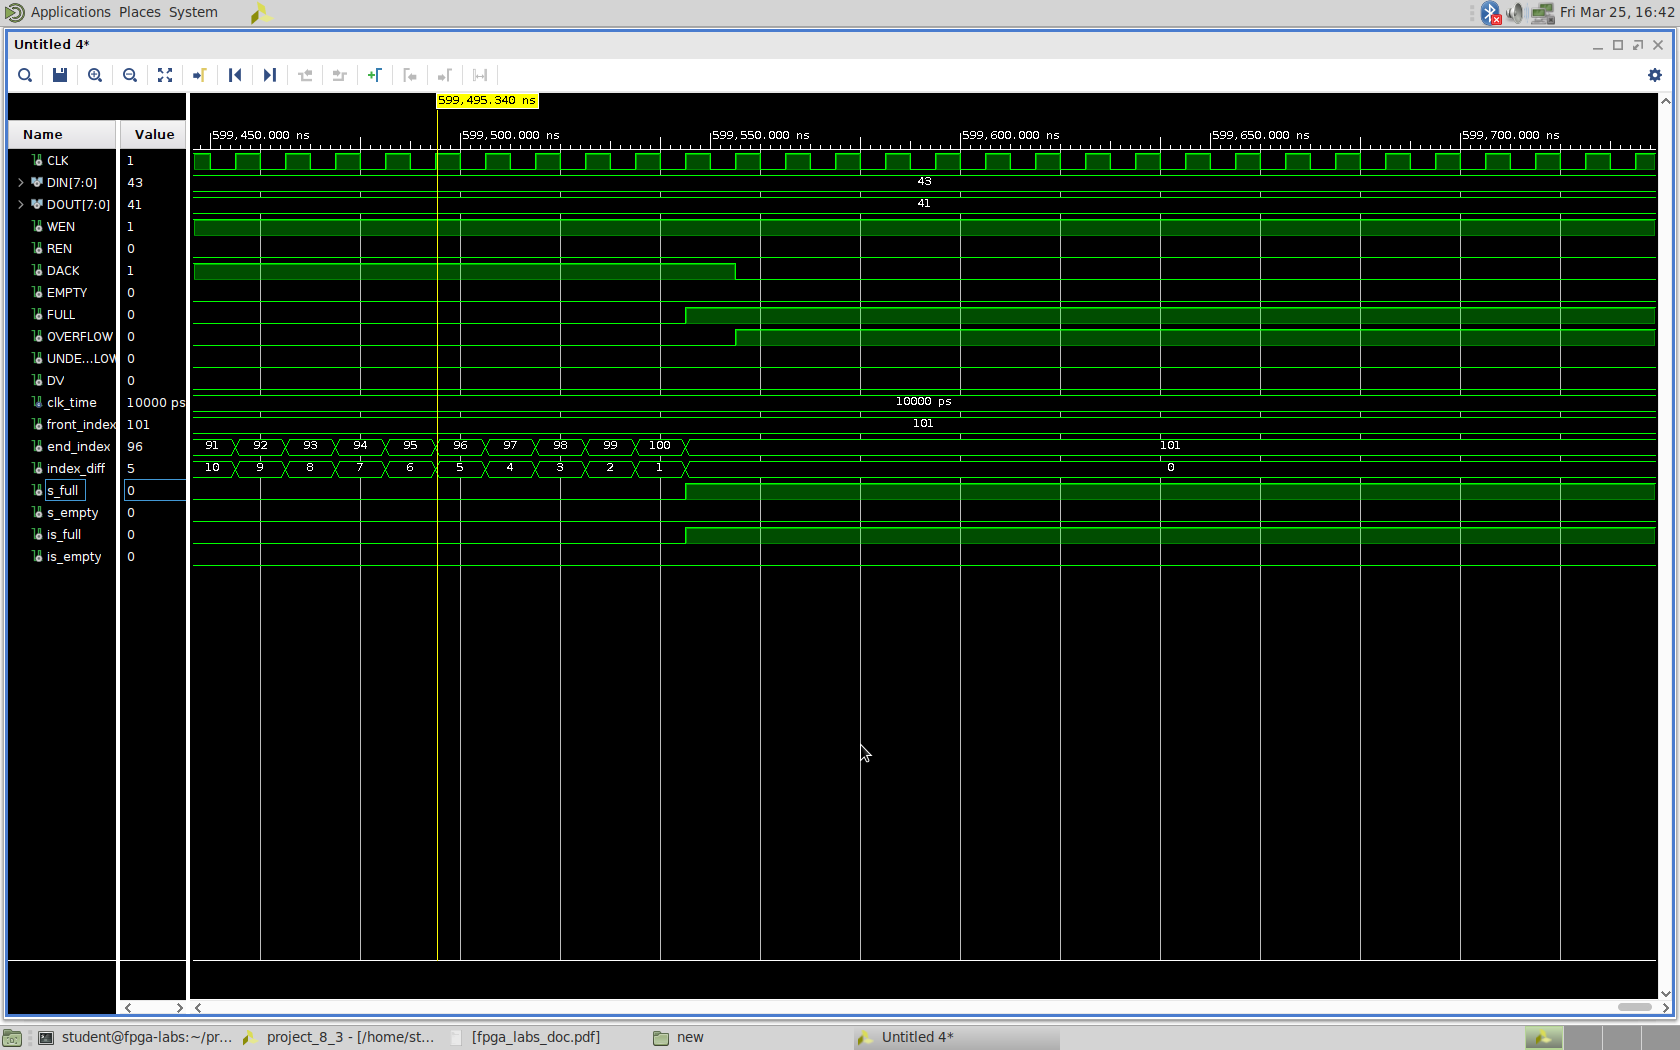
\includegraphics[width=.9\textwidth]{L8/E3/write_overflow.png}
    \caption{Writing to a full stack. The stack overflows.}
    \label{pic: r to f stack fifo}
\end{figure}